% -*- TeX-master: "Qualificacao.tex" -*-
%!TEX root = Qualificacao.tex

\chapter{Basic concepts in system identification}
\label{cap:cap2} \vspace{-1cm}

% \begin{flushright}
% \begin{minipage}{0.7\linewidth}
% \emph{``...''}
% \end{minipage}
% \end{flushright}
%
% \begin{flushright}
% {fulano}
% \end{flushright}
% \todo[inline]{Deixar claro na seção que a identificação não é feita somente por mínimos quadrados (é o que está parecendo). Apresentar outras abordagens. Apresentar outros tipos de modelos que não polinomiais (acho que isso é feito na secao de escolha do modelo, de maneira breve, mas não cito nada sobre estruturas, NARX, etc.) Deixar isso claro.  Talvez criar uma seção para modelos NARX.}
% {{{ Pequena intro
In order to describe natural phenomena or even mechanisms and processes created by the humans, over the centuries, different ways of representing such phenomena through mathematical expressions, known as mathematical models, or simply models, have been developed.

To obtain such models, in general, two approaches can be used: modeling by the first principles, or modeling by systems identification techniques. In the first case, the models are obtained from applications of laws, in general of physics, developed and documented over the years of observations of phenomena, natural or not, by scientists from the most diverse areas. In the second case, mathematical models are obtained from analyzes made on signal data collected from the system to be modeled using identification techniques developed for this purpose. In both cases, the models obtained are mathematical expressions that describe the approximate behavior of the modeled process.

In the present work, it is not of interest to obtain a model for the process, but a model for the controller. However, the methodologies used to identify systems can be used directly, or in some cases, with specific adaptations for the purpose of identifying controllers. In this sense, identification techniques used in the scope of model identification have been used in the design of data-driven controllers, targeting both linear \citep{campi2002} and non-linear \citep{campi2006} controller models.
% \todo{Está com cara que é melhor colocar este parágrafo mais para frente.}

Over the years, with the increase in the computer's processing power as well as the ease in the acquisition and storage of data, the use of techniques for identifying nonlinear models has increasingly shown to be interesting for predictions or even for better understanding of phenomena. Likewise, it is expected that non-linear controllers designed by data-oriented control techniques will often result in controllers with better performance or even greater robustness.

From a few decades ago, the task of modeling nonlinear systems has been studied, where some great works stand out \citep{billings1980,leontaritis1985,leontaritis1985a,korenberg1988,billings1989,chen1990,chen1992,aguirre1995,aguirre2000,zhu2005}.
The system identification process basically consists of the following steps: (1) Data collection; (2) Choice of model type; (3) Structure selection; (4) Estimation of parameters; (5) model validation. The following sections briefly address each of these steps.

\section{Data Collection and pre-processing} \label{sec:collection}
The first step in the identification of systems models is the data collection. In this process, some care must be taken regarding the sampling interval considered when collecting signals, from the system to be identified.  Care should also be taken when choosing the signal used to excite the process, when possible.
The input signals must be designed in such a way as to excite the dynamics of the system in the frequency range of interest, through the choice of signals with adequate spectral powers. In this case it is said that the signal must be \textit{persistently exciting}. Signals such as filtered white noise or binary pseudo-random signals (PRBS) are commonly used in practice.

The proper choice of the amplitude of the input signal is also a factor that deserves caution. For example, the signal should not be such as to cause the process response to exceed certain thresholds, close to an operating point, which guarantee a behavior close to linear in the case of the identification of linear models. Likewise, when the identification is of a non-linear model, the amplitude must be such that it explores the non-linear characteristics of the process.
Problems such as oversampling, outliers, or cases in which the excitation signals cannot be previously chosen, can be resolved or mitigated by prior treatment of the data, a process known as pre-processing.

\section{Choice of Model Class} \label{sec:choose model}

There are several model classes that can be used to describe the input-output relationship of a process. These classes have different structures that are more or less suitable for a particular application. For example, for non-linear systems, the structure of the model must be complex enough to represent the non-linearities of interest. Among the several usual classes in the representation of models, the following stand out: base radial functions \citep{broomhead1988}, neural networks \citep{haykin1994}, wavelets \citep{strang1989}, Volterra series \citep{billings1980}, polynomials and rationals functions \citep{billings1989}.

\section{Structure Selection}\label{sec:estr_selection}

Once the class of a model is defined, choosing its structure (i.e., number, degree, time lags, of terms in a NARX polynomial model) becomes the next task, before identifying its parameters.
This can be a difficult task, since we want to find a model with the lowest possible variance and polarization (bias), and these two quantities are contradictory.
% COMTEMP \todo{Encontrar palavra melhor que \textit{contraditórias}.}
In short, the model must be rich enough to capture the dynamics and repeat the behavior of the modeled system, but not so much as to model the noise present in the sampled signals.
If the model is very simple, it may not fit well with the training data, and if too complex (with many terms), it can affect the behavior prediction for data other than those used in training.

In an attempt to find a solution to this problem, approaches have been presented in recent decades.
Among them, the Akaike’s Information Criterion (AIC) gained attention, as well as its corrected version, (AICc).
The AIC, was introduced by \cite{akaike1974}, and is defined as
\begin{equation}
   AIC(n_\theta) = N \ln[\sigma^2_{\text{erro}}(n_\theta)] + 2 n _\theta
   \label{eq:AIC},
\end{equation}
where $N$ is the number of sampled data, $\sigma^2_{\text{erro}}(n_\theta)$ the variance of the residue and $n_\theta = \text{dim}[\hat {\theta}]$ the number of parameters of the model.
Bccording to \cite{aguirre2015}, \eqref{eq:AIC} can be analyzed by the following: ``Bs terms are included in the model, the number of degrees of freedom $n_d$ increases, allowing a more accurate adjustment to the data. Thus, $\sigma^2_{\text{erro}}(n_\theta)$ decreases as $n_d$ increases \dots'',
but ``\dots after a certain moment, the decrease in the variance of the residuals resulting from the inclusion of a new term is insignificant and would not justify the inclusion of the respective term ''.
In short, the first term of \eqref{eq:AIC} quantifies the decrease in the variance of the residuals due to the inclusion of a term, whereas the second term penalizes the inclusion of each term.

In order to correct a problem presented by the AIC that increases the probability of the AIC to select models with a high number of parameters when the sample size is small, which leads to an over-adjustment, the AICc appears \citep{cavanaugh1997}, given by the equation
\begin{equation}
   AICc = AIC + \frac{2k^2+2k}{n-k-1}
   \label{eq:AICc}.
\end{equation}
% COMTEMP \todo{falar um pouquinho mais sobre este caso.}

Other criteria similar to AIC can also be found in the literature, among them, the Bayesian Information Criterion (BIC), \citep{schwarz1978}; and the Final Prediction Error (FPE) \citep{kashyap1977}.

Other approaches, already considered classic, that differ from the previously mentioned criteria can be found in the literature, with emphasis on the Error Reduction Ratio (ERR) \citep{billings1989}.
In this approach, the reduction in noise variance that occurs when a new term is included in the model is quantified and normalized with respect to the output variance.
The ERR resulting from the inclusion of the i-th regressor is given by
\begin{equation}
   [\text{ERR}]_i  = \frac{MS1PE(\nu_{i-1})-MS1PE(\nu_i)}{\langle\vy,\vy\rangle}
   \label{eq:ERR},
\end{equation}
where $i = 1, 2, \dots, m$ and $m$ is the number of tested candidate terms; MS1PE$\nu_i$ the one-step ahead error of the model with $i$ terms, or regressors; and $\nu$ represents a family of models with nested structures such that $\nu_{i-1} \subset \nu_i$.
\todo{parece que faltou falar de $\vy$.}

Extensions to the ERR criterion are possible, such as ERR$_2$ \citep{alves2012}, which uses 2-steps ahead prediction instead of 1.
Another criterion similar to the ERR is the Simulation Error Reduction Ratio (SRR), introduced by \citep{piroddi2003}, and which is advantageous in non-ideal conditions, often resulting in more compact models, but with higher computational costs. It is given by
\begin{equation}
   [\text{SRR}]_i  = \frac{MSSE(\nu_{i-1})-MSSE(\nu_i)}{\langle\vy,\vy\rangle}
   \label{eq:SRR},
\end{equation}
where MSSE$\nu_i$ now represents the mean square simulation error for the model with $i$ regressors, which implies the use of free-run simulation.

More recent techniques, many of which are based on Monte Carlo approaches, have been introduced to the academic community in recent years. For the purposes of this research, the Randomized Model Structure Selection method, or simply, RaMSS \citep{falsone2014,falsone2015}, stands out.
% COMTEMP \todo[inline]{Falar um pouco mais aqui sobre RaMSS e indicar que será abordado em capítulo a parte. Estou decidindo ainda como ficará (se capítulo a parte ou se falo neste mesmo capítulo, mas talvez como uma seção a parte depois desta introdução sobre identificação).} 




\section{Parameter Estimation}%
\label{sec:parest}
% COMTEMP \todo{Aqui está parecendo que a estimação é feita exclusivamente por mínimos quadrados. Deixar claro que não. Citar outras. Criar uma seção para mínimos quadrados.} 
\todo[inline,color=green]{Acabar de traduzir daqui!} 

No processo de identificação de sistemas dinâmicos, mais especificamente utilizando estimação paramétrica, uma vez que os dados são colhidos, pré-processados e a classe do modelo e sua estrutura são escolhidos, o problema passa ser o de se determinar os melhores parâmetros para este modelo. A este processo dá-se o nome de estimação de parâmetros. O objetivo é encontrar uma função paramétrica $\hat{f}(\vvarphi_{k},\hat{\vtheta}) :  \R^{n_{\hat{\theta}}} \mapsto \R$ que se aproxime da função ideal e em geral, desconhecida, $f(\vvarphi_{k}) : \R^{n_\theta} \mapsto \R$ por meios de dados de treinamento amostrados. Desta forma
\begin{equation}
   y_k = f(\vvarphi_{k}) \approx \hat{f}(\vvarphi_{k},\hat{\vtheta}),
\end{equation}
em que $\vvarphi_{k-1} \in \R^{n_{\hat{\theta}}}$ é o vetor de regressores, formado por combinações lineares ou não lineares da saída $y_{k-1},\  \dots ,\ y_{k-n_y}$ (e.g. modelos FIR) e/ou entrada $u_{k-1},\  \dots ,\ u_{k-n_u}$ (e.g., modelos ARX, ou NARX) e até mesmo do resíduo $\xi_{k},\  \dots ,\ \xi_{k-n_\xi-1}$ (e.g., modelos ARMA, NARMAX); $\hat{\vtheta} \in \R^n_\theta$, é um vetor de parâmetros estimados; $y_k \in \R$, o sinal amostrado no instante $k$; e $n_{\hat{\theta}},\ n_y,\ n_u$  representam respectivamente: o número de parâmetros e os máximos atrasos na saída e na entrada. 

Considerando que a função ideal $f(\vvarphi_{k})$ possa ser escrita na forma paramétrica 
\begin{equation}
   y_k = f(\vvarphi_{k},\vtheta),
   \label{eq:yk}
\end{equation}
em que $\bm{\theta} \in \mathbb{R}^{n_\theta}$  é o vetor de parâmetros ideal, 
% em que $\bm{\theta} \in \mathbb{R}^{n_\theta}$  é o vetor de parâmetros ideal, esta função define um conjunto de equações, ou restrições, que pode ser reescrita, para várias observações do escalar $y$, da seguinte forma:
% \begin{align}
% \label{eq:restricoes}
%    y_k &= f(\vvarphi_{k}, \vtheta) \nonumber\\
%    y_{k-1} &= f(\vvarphi_{k-1}, \vtheta) \\
%    \vdots &= \vdots \nonumber\\
%    y_{k-N+1} &= f(\vvarphi_{k-N+1}, \vtheta),\nonumber
% \end{align}
% sendo $y_k$ a $k$-ésima observação de $y$, e $\vvarphi_{k}= \begin{bmatrix} \varphi_{k-1,k}^T & \varphi_{k-2,k} & \dots & \varphi_{k-n_\theta,k} \end{bmatrix}$\todo[color=orange]{\textbf{LAA: } Corrigir isso aqui conforme comentários do aguirre. Olhar a difinição de $\Psi$ também.} a $k$-ésima observação dos $n_\theta$ regressores no instante, ou amostra, $k$.
%
% Assumindo que $f$ é linear nos parâmetros $\vtheta$ e que tanto $f$ quanto $\vtheta$ não mudam de uma restrição para a outra em~\eqref{eq:restricoes}, pode-se escrever \eqref{eq:yk} na seguinte forma matricial
e assumindo que $f$ é linear nos parâmetros e que tanto $f$ quanto $\vtheta$ não mudam em relação ao tempo $k$, pode-se escrever \eqref{eq:yk} na seguinte forma matricial
\begin{equation}
   \label{eq:yMatrix}
   \vy = \Psi\bm{\theta},
\end{equation}
em que $\Psi = \begin{bmatrix} \vvarphi_{k} & \vvarphi_{k-1} & \dots & \vvarphi_ {k-N+1} \end{bmatrix}^T$ e $\vy = \begin{bmatrix} y_k & y_{k-1} & \dots & y_{k-N+1} \end{bmatrix}^T$.

% A solução deste problema pode ser encontrada a partir do método dos mínimos quadrados

Se $N=n_\theta$ restrições, o vetor de parâmetros $\vtheta$ pode ser determinado por
\begin{equation}
   \vtheta = \Psi^{-1}\vy
   \label{eq:thetaest}.
\end{equation}

Porém se $N > n_\theta$ restrições são tomadas, o sistema é dito sobre-determinado e a matrix $X$ passa a ser não quadrada e não invertível. Uma solução é reescrever \eqref{eq:yMatrix} de forma que a solução não seja exata, a partir da introdução de um termo de erro $\bm{\xi} \in \mathbb{R}^N$, conhecido como vetor de \emph{resíduos}, resultando em
\begin{equation} 
   \label{eq:ysobredet}
   \vy =  \Psi\hat{\vtheta} + \vxi.
\end{equation}

Para que o modelo capture o comportamento do processo modelado, é intuitivo que o vetor de parâmetros estimados $\hat{\vtheta}$ seja escolhido de forma que $\vxi$ seja reduzido em algum sentido. Na estratégia conhecida como Mínimos Quadrados Ordinário ou, simplesmente, mínimos quadrados ou LS (do inglês Least Squares), uma função de custo relacionada ao vetor de resíduos é definida como
\begin{equation}
   \label{eq:JLS}
   J_{LS} = \sum_{k=1}^{N} \vxi(k)^2 = \vxi^T\vxi = ||\vxi||^2.
\end{equation}
Prova-se que o vetor $\hat{\vtheta}_{LS}$, definido como o conjunto de parâmetros que minimiza $J_{LS}$ pode ser calculado por meio da pseudo-inversa de $\Psi$, de forma que \citep{aguirre2015}:
\begin{equation}
   \hat{\vtheta}_{LS} = [\Psi^T \Psi]^{-1}\Psi^T \vy.
   \label{eq:LS}
\end{equation}
A equação \eqref{eq:LS} representa o estimador dos mínimos quadrados, onde os parâmetros são determinados pela minimização da função de custo referente ao somatório do quadrado dos erros de modelagem.
Alternativas numéricas mais interessantes que o algorítimo clássico de \eqref{eq:LS} podem ser encontradas \citep{aguirre2015,ljung1999}, porém o fundamento básico permanece o mesmo.


\section{Model Validation}\label{sec:model_validation}

Tendo sido estimados os parâmetros que minimizam o resíduo em algum sentido, como por exemplo em função do somatório do quadrado dos erros de modelagem, caso dos mínimos quadrados apresentado em \eqref{eq:LS}, deve-se avaliar o desempenho do modelo quando este estiver sujeito a excitações diferentes daquelas submetidas durante o processo de identificação (treinamento). 

Para  isso, é comum utilizar-se de um conjunto de dados amostrados diferente daquele usado no processo de identificação. A este conjunto de dados dá-se o nome de conjunto de validação. É usual colher-se uma certa quantidade de dados do processo, sujeito a um sinal de excitação adequado, e posteriormente dividir o conjunto de dados resultante em um conjunto de treinamento e outro de validação.

O passo seguinte consiste em utilizar-se de algum índice de desempenho de forma a quantificar a qualidade da previsão em um teste conhecido como \textit{free-run simulation}. Nessa simulação, o modelo obtido no processo de identificação é submetido ao mesmo sinal de excitação sob o qual fora submetido o conjunto de validação. Os resultados simulados e colhidos armazenados previamente são então comparados a partir de alguma métrica. Dentre as métricas mais usuais, destacam-se o \textit{Mean Square Error} (MSE) e a \textit{Mean Absolute Percentage Error} (MAPE).

O MSE é dado por
\begin{equation}
   \label{eq:MSE}
   \text{MSE} = \frac{1}{N}\sum_{k=1}^{N}(y_k-\hat{y}_k)^2,
\end{equation}
sendo $M$ o número de amostras, $y_k$ o dado amostrado no intervalo $k$ e $\hat{y}_k$ a predição do modelo. O MSE pode ser calculado tanto sobre os dados de treinamento quanto sobre dados de validação. Porém, para fins de validação, os dados de validação devem ser utilizados, umas vez que assim pode-se obter uma medida do desempenho para o modelo se comportando fora do ambiente de treinamento. Um bom modelo, em geral, deve apresentar o MSE sobre os dados de validação próximo ao MSE sobre os dados de treinamento. 

Baseados no MSE, definem-se dois outros índices de desempenho: o \textit{Mean Square Prediction Error}, ou MSPE, e o \textit{Mean Square Simulation Error}, ou MSSE.
O MSPE é definido como o MSE utilizando como dados de predição do modelo $\hat{y}_k$ dados de predição um passo a frente. Já o MSSE, utiliza dados de simulação livre como dados de predição $\hat{y}_k$ nos cálculos. Versões modificadas do MSPE podem ser também usadas, como o MS2PE, que utiliza predição de 2 passos a frente.

O MAPE, por sua vez, calcula o desvio absoluto da predição em relação aos dados observados e é, em geral, calculado em porcentagem, na forma
\begin{equation}
   \label{eq:MAPE}
   % \text{MAPE} =  \frac{100\%}{N}\sum_{k=1}^{N} \frac{|y_k - \hat{y}_k|}{|\max(y_k)-\min(y_k)|}. % Petrus
   \text{MAPE} =  \frac{100}{N{\sigma(\bm{y})}}\sum_{k=1}^{N} {|y_k - \hat{y}_k|}\ \%, % Codigo Aguirre
\end{equation}
em que $\bm{y}=[y_1,\ y_2,\ \dots,\ y_N]^T$ e $\sigma(\bm{y})$ representa o desvio padrão de $\bm{y}$. 

Diferentes formas de escolha dos dados de treinamento e validação em relação à usual apresentada em \eqref{eq:MAPE} podem ser usados.
% , como por exemplo, quando escolhe-se metade dos dados, ou conjuntos proporcionais.
Uma destas formas é a “leave-one-out cross-validation”, em que apenas um dado, de todo o conjunto de dados é usado de cada vez \citep{allen1974}.
% \todo{Melhorar um pouco.} % Acho que esta ok agora, mexi.

Além da validação quantitativa em geral recorre-se ainda a uma avaliação qualitativa, na qual é realizada uma comparação gráfica, quanto ao comportamento dinâmico, entre a curva do sinal amostrado e a curva do sinal estimado pelo modelo resultante.
\todo{Melhorar este final}

%!TEX root = Qualificacao.tex

\section{Randomized Model Structure Selection}%
\label{sec:ramss}

% COMTEMP \todo[inline]{Coloquei o RaMSS por enquanto nesta seção, mas estou querendo colocar em um capítulo a parte. Só mencioná-lo na seção anterior como método de seleção de estrutura. No capítulo a parte colocarei uma introdução sobre métodos estatísticos e teria ainda espaço para exemplos de aplicação do RaMSS para identificação de sistemas (processos). Mai a frente abordaria o uso para identificação de controladores.} 

% O método RaMSS, apresenta uma abordagem alearorizada para escolha de uma estrutura de modelo adequada por meio da amostragem de modelos de um conjunto de modelos $\mathscr{M}$.
The RaMMS method presents a randomized approach for choosing an appropriate model structure by sampling models from a set of models $\mathscr{M}$.
% Introduzido por \cite{falsone2014} e aperfeiçoado em \cite{falsone2015}, o método realiza a tarefa de seleção de estrutura de maneira probabilística que, apesar do caráter aleatório, evita a busca exaustiva necessária para analisar todos os regressores do conjunto de regressores candidatos, definido por $\mathscr{R}$,
Introduced by \cite{falsone2014} and improved in \cite{falsone2015}, the method performs the task of  structure selection in a probabilistic way that, despite the random behavior, avoids the exhaustive search necessary to analyze all the possible models in the set of candidate regressors, defined by $\mathscr{R}$,
% COMTEMP \todo{tentar colocar isso (a definição do conjunto) de uma maneira mais formal (fórmula).} 
% que seria necessário ao se utilizar força bruta em uma estratégia puramente Monte Carlo.
that would be needed when using brute force in a purely Monte Carlo strategy.

% O método procura iterativamente pelo melhor subconjunto de regressores no conjunto $\mathscr{R}$ visando maximizar a acurácia da predição do modelo segundo um índice definido. Isto é feito através de modelos candidatos, subconjuntos de $\mathscr{M}$, construídos a partir de regressores amostrados do conjunto $\mathscr{R}$ com a probabilidade de escolha dada por uma função de probabilidade estimada chamada de RIP (\textit{Regressor Inclusion Probability})
Considering a set of all possible models formed by $\mathscr{R}$, named universe set and represented by $\mathscr{U}$, the method iteratively searches for the best subset of regressors in the $\mathscr{R}$ set in order to maximize the accuracy of the model's prediction according to a defined index. This is done by a set of candidate models, defined as $\mathscr{M} \in \mathscr{U}$, built from regressors sampled from the $\mathscr{R}$ set with a probability of choice given by an estimated probability function called RIP (\textit{Regressor Inclusion Probability}).

% Uma vez escolhido um modelo candidato, este é avaliado de acordo com algum critério de desempenho e os RIP são atualizados. A cada iteração, $N_p$ modelos são tomados de $\mathscr{M}$ e índices de desempenho são calculados para a atualização dos RIP.
Once a candidate model is chosen, it is evaluated according to some performance criteria and the RIPs are updated. At each iteration, $N_p$ models are taken from $\mathscr{U}$ set and performance indexes are calculated for updating the RIPs.
% Estes índices são, em geral,  baseados no MSPE, MSSE ou uma combinação dos dois, e são usados para calcular um índice médio de desempenho do regressor avaliado.

These indexes are, in general, based on the MSPE, MSSE or a combination of the two, and are used to calculate an average performance index $\mathcal{I}$ of the evaluated regressor.
% Assumindo um conjunto $\mathscr{M}$ de $N_p = \dim(\mathscr{M})$ modelos em que alguns contêm o $j$-ésimo regressor, um índice que mensura o \textit{desempenho médio do regressor}, que pode ser usado no cálculo do RIP é definido como
Assuming a set $\mathscr{M}$ of $N_p = \dim(\mathscr{M})$ models, where some contain the $j$-th regressor (and others possibly not), an index that measures the \textit{average performance of the regressor}, which can be used in calculating the RIP is defined as
\begin{align}
   \mathcal{I}_j &= \mathcal{I}_j^+ - \mathcal{I}_j^- \nonumber\\
      % &= \E[\mathcal{J}^{+}_{j}] - \E[\mathcal{J}^{-}_{j}]
      &= \E[\mathcal{J}(\mathscr{M})|\phi_j \in \mathscr{M}] - \E[\mathcal{J}(\mathscr{M})|\phi_j \notin \mathscr{M}],
\label{eq:desMedioReg}
\end{align}
% COMTEMP \todo{decidir aqui: usar $\mathscr{M}$ ou  $ \mathscr{R}$ -- eq. \eqref{eq:desMedioReg}.}
% sendo $j = 1,\ \dots,\ m$, em que  $m = \dim{(\mathscr{R})}$ é o número de regressores considerados, $\mathcal{J}(\mathscr{M})$ representa o vetor contendo os índices de desempenho para os modelos escolhidos, $\mathscr{M}$ é o conjunto de regressores candidatos, $\phi_j$ o $j$-ésimo regressor e $\E[\cdot]$ é o operador de esperança matemática\footnote{Caso o evento condicional tenha probabilidade nula de ocorrer, a esperança é assumida nula.}. Desta forma, o índice de desempenho $\mathcal{I}_j$ compara o desempenho médio dos modelos contendo o $j$-ésimo regressor ($ \mathcal{I}_j^+$) com o desempenho dos modelos que não contêm este mesmo regressor ($ \mathcal{I}_j^+$).
being $j = 1,\ \dots,\ m$, where $m = \dim{(\mathscr{R})}$ is the number of regressors considered, $\mathcal{J}(\mathscr{M})$ represents the vector containing the performance indexes for the chosen models, $\mathscr{M}$ is the set of candidate regressors, $\phi_j$ the $j$-th regressor and $\E[\cdot]$ is the operator of mathematical expectation\footnote{If the conditional event has zero probability of occurring, expectation is assumed to be null.}. Thus, the performance index $\mathcal{I}_j$ compares the average performance of models containing the $j$-th regressor ($ \mathcal{I}_j^+$) with the performance of models that do not contain this same regressor ($ \mathcal{I}_j^+$).
% Como em geral a esperança matemática da equação \eqref{eq:desMedioReg} não pode ser calculada de forma analítica, esta é, na prática, feita por estimação, tomando modelos do modelo universo $\mathscr{U}$ e calculando a média amostral, resultando em
As, in general, the mathematical expectation of the equation \eqref{eq:desMedioReg} cannot be calculated analytically, this is done, in practice, by estimation, taking models from the universe model $\mathscr{U}$ set and calculating the sample mean, resulting in
\begin{equation}
   \mathcal{I}^+_j = \frac{1}{n_j^+}\sum_{i \in \mathscr{M}_j^+}\mathcal{J}^{+}_{i} \qquad \text{e} \qquad \mathcal{I}^-_j = \frac{1}{n_j^-}\sum_{i \in \mathscr{M}_j^-}\mathcal{J}^{-}_{i},
\label{eq:avgRefPerf}
\end{equation}

% onde $ \mathscr{M}^+_j \subset \mathscr{M}$ e $ \mathscr{M}^+_j \subset \mathscr{M}$, representam os conjuntos de todos os modelos que, respectivamente, contêm e não contêm o $j$-ésimo regressor $\phi_j$, com $n_j^+ = \dim \mathscr{M}^+_j $ e $n_j^- = \dim \mathscr{M}^-_j$. Os termos $\mathcal{J}^{+}_{i}$ e  $\mathcal{J}^{-}_{i}$ representam os respectivos índices de desempenho para os casos que contêm e que não contêm $\phi_j$.

where $ \mathscr{M}^+_j \subset \mathscr{M}$ and $ \mathscr{M}^+_j \subset \mathscr{M}$, represent the sets of all models that, respectively, contain and do not contain the $j$-th regressor $\phi_j$, with $n_j^+ = \dim \mathscr{M}^+_j $ and $n_j^- = \dim \mathscr{M}^-_j $. The terms $\mathcal{J}^{+}_{i}$ and $\mathcal{J}^{-}_{i}$ represent the respective performance indexes for cases that contain and do not contain $\phi_j$.



% Assumindo que o modelo real definido por $f^*$, o qual se deseja encontrar, pertence ao conjunto de todas as possíveis estruturas (conjunto universo) $\mathscr{M}$, deve ser possível achar este modelo explorando o conjunto de modelos $\mathscr{M}$ e tomando os modelos com melhor desempenho.  O problema de se achar o modelo real em função de um índice pode ser representado por
Assuming that the actual model, defined by $f^*$, belongs to the set of all possible structures (universe set) $\mathscr{U}$, it must be possible to find this model by exploring the set of models $\mathscr{M}$ and taking the models with the best performance. The problem of finding the real model as a function of an index can be represented by
\begin{equation}
   f^* = \argmax_{\tilde{f} \in \tilde{\mathscr{U}}} \mathcal{J}(\tilde{f}),
\label{eq:fStar}
\end{equation}
% onde $ \mathcal{J}$ é algum\footnote{A definição de $\mathcal{J}$ adotada na proposta original do RaMSS é apresentada mais adiante no texto (vide eqs. \ref{eq:Jp} a \ref{eq:Jcal}). } índice de desempenho calculado para os modelos candidatos $\tilde{f}$ tomados do conjunto universo não redundante  $\tilde{\mathscr{M}} \subset{\mathscr{M}}$\footnote{Note que no conjunto universo é comum o aparecimento de modelos redundantes, oev  seja, modelos similares que não incluem termos estatisticamente relevantes. Na prática é comum que estes sejam removidos e a amostragem seja realizada em um conjunto reduzido do modelo universo, definido por $\tilde{\mathscr{M}} \subset \mathscr{M}$.}, ou   mesmo por $ \mathscr{M}$.
where $ \mathcal{J}$ is some\footnote{The definition of $\mathcal{J}$ adopted in the original proposal of RaMSS is presented later in the text (see eqs. \ref{eq:Jp} a \ref{eq:Jcal}). } performance index calculated for candidate models $\tilde{f}$ taken from the non-redundant universe set $\tilde{\mathscr{U}} \subset{\mathscr{U}}$\footnote {Note that in the universe set it is common for redundant models to appear, ie, similar models that do not include statistically relevant terms. In practice, it is common for these to be removed and sampling to be performed on a reduced set of the universe model, defined by $\tilde{\mathscr{U}} \subset \mathscr{U}$.}, or even by $ \mathscr{U}$.


% No sentido de achar a estrutura correta do modelo, ou seja $ f^*$, o algoritmo RaMSS amostra $N_p$ modelos de $ \mathscr{M}$, calcula o desempenho $\mathcal{J}(\tilde{f})$ para cada modelo candidato $\hat{f}_{i}$, com $i=1,\ \dots,\ N_p$ e estima a média sobre todos os modelos que envolvem o regressor $\phi_j$. Isto é feito para cada um dos $m=\dim(\mathscr{R})$ regressores do conjunto $\mathscr{R}$ de regressores candidatos.
In order to find the correct model structure, i.e. $ f^*$, the RaMSS algorithm samples $N_p$ models from $ \mathscr{U}$, calculates the performance index $\mathcal{J}(\tilde{f})$ for each candidate model $\hat{f}_{i}$, with $i=1,\ \dots,\ N_p$ and estimates the average over all models involving the $\phi_j$-th regressor. This is done for each of the $m=\dim(\mathscr{R})$ regressors of the $\mathscr{R}$ set of regressors.

% Considerando que o índice de desempenho $\mathcal{J}$ em \eqref{eq:fStar} tenha valores no intervalo $[0,\ 1]$, i.e.  $ \mathcal{J}(\tilde{f}) \in \R : \mathcal{J}(\tilde{f}) \in [0,\ 1] $
Considering that the performance index $\mathcal{J}$ in \eqref{eq:fStar} has values in the $[0,\ 1]$ range, i.e. $ \mathcal{J}(\tilde{f}) \in \R : \mathcal{J}(\tilde{f}) \in [0,\ 1] $
\todo{Confirmar isso aqui}, 
% o valor esperado de $\mathcal{J}$,
% seu valor esperado, considerando $ \mathcal{P}$ a distribuição de probabilidade ao se escolher o regressor $\phi_j$ como variável aleatória $\mathscr{M}$ na realização de uma amostra de modelo em  $ \tilde{\mathscr{M}}$, será dado por
its expected value, considering the probability distribution  $ \mathcal{P}$ and a random variable $\Phi \equiv \tilde{\mathscr{M}}$ that corresponds to a realization a model sample in $ \tilde{\mathscr{U}}$, will be given by
\begin{equation}
  \E[\mathcal{J}] = \sum_{\tilde{f}\in \tilde{\mathscr{U}}} \mathcal{J}(\tilde{f})\mathcal{P}(\mathscr{U}=\tilde{f})
\label{eq:espJ}
\end{equation}

% Se $\mathcal{P}$ é variado sobre todas as possíveis distribuições em $\tilde{\mathscr{U}}$, o máximo de \eqref{eq:espJ} é obtido ao se concentrar toda a massa de probabilidade no modelo mais adequado. Com isso, a solução do problema de otimização pode é obtida por
If $\mathcal{P}$ is varied over all possible distributions in $\tilde{\mathscr{U}}$, the maximum of \eqref{eq:espJ} is obtained by concentrating the entire probability mass on the most appropriate model. With that, the solution to the optimization problem can be obtained by
\begin{equation}
   \mathcal{P}^* = \argmax_{\Phi\in  \tilde{\mathscr{U}}} \E\left[ \mathcal{J}(\Phi)  \right]   
\label{eq:Pargmax}
\end{equation}
% e é tal que $\mathcal{P}=1$. Assim, resolvendo \eqref{eq:Pargmax} seleciona-se o modelo mais adequado, ou modelo real $f^*$, com a mesma solução de \eqref{eq:fStar}.
and it's such that $\mathcal{P}=1$. Thus, by solving \eqref{eq:Pargmax}, the most appropriate model, or real model $f^*$, is selected with the same solution as \eqref{eq:fStar}.

% O método RaMSS estima $\mathcal{P}$ e, consequentemente, o melhor modelo como se segue. A cada iteração, $N_p$ modelos candidatos são montados a partir de $m$ regressores candidatos. A escolha de cada regressor $\phi_j$ componente de um modelo candidato é feita a partir de um processo de Bernoulli, por uma variável aleatória associada a cada regressor  $\phi_j$ tal que
The RaMSS method estimates $\mathcal{P}$ and, consequently, the best model as follows. At each iteration, $N_p$ candidate models are assembled from $m$ candidate regressors. The choice of each $\phi_j$ regressor component of a candidate model is made based on a Bernoulli process, by a random variable associated with each $\phi_j$ regressor such that
\begin{equation}
   \rho \approx \text{Be}(\mu_j),
\label{eq:bernulli}
\end{equation}
% onde possíveis resultados são: 1, com probabilidade (de sucesso) $\mu_j$ de ocorrer; e 0, com probabilidade $(1-\mu_j)$; sendo $\mu_j \in [0,\ 1]$,  com $ j=1, \dots, m$ e $m$ o número de regressores candidatos.
where possible results are: $\rho=1$, with $\mu_j$ probability (of success) to occur; and $\rho=0$, with probability $\mu_j$; where $\mu_j \in [0,\ 1]$, with $ j=1, \dots, m$ and $m$ the number of candidate regressors.
% Caso $\rho=1$, o regressor  $\phi_j$ estará presente no modelo candidato construído, caso contrário, não.
If $\rho=1$, the $\phi_j$ regressor will be present in the candidate model built, otherwise, no.

% Assume-se que variáveis aleatórias $\rho_j$ são independentes\footnote{Apesar de existirem resultados na literatura \citep{bianchi2016} sugerindo que uma abordagem utilizando distribuição Bernoulli condicionada e multivariada pode resultar em melhorias na acurácia do processo de seleção de modelos, um procedimento inicial adotado neste trabalho considera independência.} e define-se um vetor $\bm{\mu} = [\mu_1,\ \mu_2,\ \dots,\ \mu_m]^T$ como o vetor de \textit{Probabilidade de Inclusão de Regressor} (RIP). Note que o RIP, ou $\vmu$ é quem dita a distribuição de probabilidade  $ \mathcal{P}$ sobre os modelos em $\tilde{\mathscr{M}}$ (ou $\mathscr{M}$), ou seja, dado um $\bm{\mu}$ conhecido, a probabilidade de se obter um modelo de estrutura $\tilde{f}$ em qualquer subconjunto de $n_\theta$ regressores será
It is assumed that $\rho_j$ random variables are independent \footnote{Although there are results in the literature \citep{bianchi2016} suggesting that an approach using conditioned and multivariate Bernoulli distribution may result in improvements in the accuracy of the model selection process, an initial procedure adopted in this work considers independence.} and a $\bm{\mu} = [\mu_1,\ \mu_2,\ \dots,\ \mu_m]^T$ vector is defined as the vector of \textit{Probability of Inclusion of Regressor} (RIP). Note that the RIP, or $\vmu$, is the one that dictates the $ \mathcal{P}$ probability distribution on the models in $\tilde{\mathscr{U}}$ (or $\mathscr{U}$), that is, given a known $\bm{\mu}$, the probability of obtaining a $\tilde{f}$ structure model in any subset of $n_\theta$ regressors is
\begin{equation}
   \mathcal{P}(\tilde{f}) = \prod_{j:\phi_j \in \tilde{f}}^{n_{\theta}} \mu_j \prod_{j:\phi_j \notin \tilde{f}}^{m-n_{\theta}} (1-\mu_j),
\label{eq:distProbf_til}
\end{equation}
to any $ \tilde{f} \in \tilde{\mathscr{U}}$.

% O procedimento é executado de modo que a cada iteração os regressores são escolhidos de acordo com o processo de Bernoulli, onde a probablilidade de escolha $\mu_j$ de cada regressor $\phi_j$ é representada pelo vetor de RIP. O vetor de RIP, $\bm{\mu}$ é refinado por sucessivas iterações de uma regra de atualização definida como
The procedure is performed so that at each iteration the regressors are chosen according to the Bernoulli process, where the probability of choosing $\mu_j$ for each $\phi_j$ regressor is represented by the RIP vector. The RIP vector, $\bm{\mu}$ is refined by successive iterations of an update rule defined as
\begin{equation}
   \mu_j(i+1) = \mu_j(i) + \gamma \mathcal{I}_j,
\label{eq:RIPupdate}
\end{equation}
% onde $\gamma$ é um parâmetro de projeto, $I_j$ o índice de desempenho definido em \eqref{eq:desMedioReg} e $i$ o índice da iteração do algoritmo.
where $\gamma$ is a project parameter, $\phi_j$ the performance index defined in \eqref{eq:desMedioReg} and $i$ the index of the algorithm's iteration.

% \vspace{2cm} \hrulefill

% Depois de algumas iterações é esperado que os desempenhos médios dos modelos que contém os regressores certos fiquem significantemente maiores que os que não contém, fazendo com que os regressores ``corretos'' sejam mais prováveis de serem incluídos no modelo final. O método não garante que $ \bm{\mu}$ será limitado. Para evitar que os valores do RIP cresçam, ou decresçam indefinidamente, uma saturação dos elementos em uma faixa com valor mínimo maior ou igual a 0, e máxima, menor ou igual a 1, é aplicada pelo algoritmo.
After a few iterations, it is expected that the average performances of the models containing the right regressors will be significantly higher than those that do not, making the correct regressors more likely to be included in the final model. The method does not guarantee that $ \bm{\mu}$ will be limited. To prevent the RIP values from increasing, or decreasing indefinitely, a saturation of the elements in a range with a minimum value greater than or equal to 0, and a maximum value less than or equal to 1, is applied by the algorithm.

% O parâmetro de projeto $\gamma$, de  \eqref{eq:RIPupdate} é escolhido de forma a controlar a velocidade de convergência. Valores maiores tendem a levar a uma convergência mais rápida mas pode também levar a não convergência do método. Para lidar com este problema de convergência, \cite{falsone2015} propõem um parâmetro adaptativo, dado por
The project parameter $\gamma$, from \eqref{eq:RIPupdate} is chosen in order to control the convergence speed. Larger values tend to lead to faster convergence but it can also lead to non-convergence of the method. To deal with this convergence problem, \cite{falsone2015} proposes an adaptive parameter, given by
\begin{equation}
   \gamma = \frac{1}{10(\mathcal{J}_{\max}- \bar{\mathcal{J}}) + 0.1}, 
\label{eq:gamma}
\end{equation}
% onde $\mathcal{J}_{\max}$ representa o índice de desempenho do melhor modelo e $\bar{\mathcal{J}}$ representa o índice de desempenho médio na iteração corrente.
where $\mathcal{J}_{\max}$ represents the performance index of the best model and $\bar{\mathcal{J}}$ represents the average performance index in the current iteration.
% A proposta do passo adaptativo é de que, se $\bar{\mathcal{J}}$ está longe do melhor índice de desempenho, $\gamma$ é feito pequeno de modo a compensar a grande variância provável daquela população de modelos. Porém, se  $\bar{\mathcal{J}}$ é próximo de $\mathcal{J}_{\max}$, os modelos amostrados têm baixa variância de desempenho, o que indica que o RIP deve ser atualizado em maior valor.
The purpose of the adaptive step is that, if $\bar{\mathcal{J}}$ is far from the best performance index, $\gamma$ is made small in order to compensate for the large probable variance of that model population. However, if $\bar{\mathcal{J}}$ is close to $\mathcal{J}_{\max}$, the sampled models have low performance variance, which indicates that the RIP should be updated to a greater value.

% O método RaMSS, como apresentado originalmente pelos autores, utiliza como base para o cálculo do índice de desmpenho $\mathcal{J}$, grandezas relacionadas ao MSPE e ao MSSE, definidos na seção \ref{sec:model_validation}. O índice de desempenho médio é calculado como um valor exponencial destes índices ponderados por um ganho $K$, utilizado como parâmetro de projeto. Desta forma tem-se,
The RaMSS method, as originally presented by the authors, uses as basis for calculating the performance index $\mathcal{J}$, quantities related to MSPE and MSSE, defined in the Section \ref{sec:model_validation}. The average performance index is calculated as an exponential value of these indices weighted by a $K$ gain, used as a design parameter. This way,
\begin{align}
  \mathcal{J}_p = e^{-K\cdot MSPE}, \label{eq:Jp} \\
  \mathcal{J}_s = e^{-K\cdot MSSE}. \label{eq:Js}
\end{align}
% Note que $\mathcal{J}_p$ e $\mathcal{J}_s$ terão valores no intervalo $[0 \ 1]$, onde valores próximos a 1 correspondem a um melhor desempenho, e próximos a 0, a piores desempenhos.
Note that $\mathcal{J}_p$ and $\mathcal{J}_s$ will have values in the $[0 \ 1]$ range, where values close to 1 correspond to better performance, and close to 0, worse performance. The $K$ parameter defines the sensitivity of the performance index, where the difference between models is amplified to values greater than $K$.

% O valor final de $\mathcal{J}$ é calculado como
The final value of $\mathcal{J}$ is calculated as
\begin{equation}
  \mathcal{J} = \alpha \mathcal{J}_s + (1-\alpha)\mathcal{J}_p
\label{eq:Jcal}
\end{equation}
% onde $\alpha \in [0 \ 1]$ é um parâmetro definido pelo projetista. O parâmetro $K$ define a sensibilidade do índice de desempenho, onde a diferença entre modelos é amplificada para valores maiores de $K$.
where $\alpha \in [0 \ 1]$ is a parameter defined by the designer. 

% COMTEMP \todo[inline, color=red]{Continuar aqui!??}

% TODO: [DONE] {Colocar aqui sobre $\mathcal{J}$, como é definido, etc.}

% Passadas algumas iterações o espera-se que vetor de RIP, $\bm{\mu}$, convirja para uma distribuição de equilíbrio. O modelo final será o modelo correto esperado do sistema e será composto pelos regressores associados aos RIP com valores maiores que certo limiar definido pelo projetista. Assumindo-se que o modelo real $f^* \in \tilde{\mathscr{M}}$, este limiar em geral é ajustado para um valor próximo a 1.
After a few iterations, the RIP vector, $\bm{\mu}$, is expected to converge to an equilibrium distribution. The final model will be the correct model expected from the system and will consist of regressors associated with RIPs with values greater than a certain threshold defined by the designer. Assuming that the real model $f^* \in \tilde{\mathscr{U}}$, this threshold is generally set to a value close to 1.

% O pseudo-código para o método RaMSS descrito é apresentado no Algorithm \ref{alg:RaMSS}. Na sequência é apresentado  um exemplo para identificação de sistema utilizando o  método.
The pseudo-code for the described RaMSS method is presented in Algorithm \ref{alg:RaMSS}. Following is an example for system identification using the method.
    % \For(\tcp*[f]{Start Policy Improvement}){each $\vx_k \in \Omega_k$}

\begin{algorithm}[htpb]
  \caption{RaMSS algorithm}\label{alg:RaMSS}
  $\bm{y},N_p,m,\mu_{\min},\mu_{\max},K,\mathscr{M}=\{\phi_{1},\dots,\phi_{m}\}$ \\
  \While{$iter < iter_{\max}$} 
   {
     $ \bm{\mu} \gets \bm{\mu}_0$
     \For(\tcp*[f]{Model Sampling}){$i=1:N_p$}
      {
         $\tau \gets 0$ \\
         $\bm{\psi}(k) \gets [\ ]$ \tcp*[f]{Initialize model} \\
         \For{$i=1:m$}
         {
           $r_j \gets \text{Be}(\mu_j)$ \tcp*[f]{Sample from a Bernoulli distribution}\\
            \If{$r_j = 1$}
            {
            $\bm{\psi}(k) \gets \begin{bmatrix} \bm{\psi}^T(k) & \phi_j \end{bmatrix}^T $ \\
            $\tau \gets \tau + 1$ \\
            }
         }
         \For{$h=1:\tau$}
         {
           $\tilde{\bm{\psi}}(k) \gets \text{non-redundant}(\bm{\psi(k)})$ \tcp*[f]{Remove redundant terms}\\
         }
         $\hat{\bm{y}} \gets \text{Predict}(\tilde{\bm{\psi}}(k))$ \\
         $\mathcal{J}_i \gets e^{-K\cdot MSPE(\bm{y},\bm{\hat{y}})} $
      }
      \For(\tcp*[f]{RIP Update}){$j=1:m$}
      {
         $\mathcal{J}^{+} \gets 0$; $ \mathcal{J}^{-}$; $n^{+} \gets 0$; $n^{-} \gets 0$; \\
         \For{$i=1:N_p$}
         {
            \If{$\phi_j(k) \in \tilde{\bm{\psi}}(k)$}
            {
               $\mathcal{J}^{+} \gets \mathcal{J}^{+} + \mathcal{J}_i$ \\
               $n^{+} \gets n^{+} + 1$
            } \Else
            {
               $\mathcal{J}^{-} \gets \mathcal{J}^{-} + \mathcal{J}_i$ \\
               $n^{-} \gets n^{-} + 1$
            }
            $\mathcal{I}_j \gets \left( \frac{\mathcal{J}^{+}}{\max(n^+,1)} \frac{\mathcal{J}^{-}}{\max(n^-,1)} \right) $ \\
         $\mu_j \gets \mu_j + \gamma \mathcal{I}_j$ \\
         $\mu_j \gets \max \left( \min(\mu_j, \mu_{\max}), \mu_{\min} \right) $ \\
         }
      }
   }
\end{algorithm}%[H]

\begin{exmp}[Idendificação de um modelo não-linear utilizando o RaMSS]
  \label{ex:varHeater}
  % Como exemplo ilustrativo da utilização do algoritmo RaMSS na escolha de estrutura e identificação de sistemas é usado um modelo de um pequeno aquecedor elétrico, com dissipação variável. A variação da dissipação é resultado do acionamento de um ventilador. O sinal de entrada é a tensão elétrica aplicada ao aquecedor e a saída é o sinal amplificado de um termopar. Mais detalhes sobre este modelo podem ser encontrados em \citep{aguirre2015}, seção 16.6.

  % Como exemplo ilustrativo da utilização do algoritmo RaMSS na escolha de estrutura e identificação de sistemas é usado um modelo não linear fornecido em \cite{baldacchino2013}, dado por:
  As an illustrative example of the use of the RaMSS algorithm in the structure selection, consider a nonlinear model provided in \cite{baldacchino2013}, given by:
  \begin{equation}
    y(k) = 0.7y(k-1)u(k-2) - 0.5y(k-2) + 0.6u^2(k-2) - 0.7y(k-2)u^2(k-2) + e(k)
  \label{eq:}
  \end{equation}
  % sendo o sinal de excitação $u(k)$ adotado como um sinal com distribuição uniforme entre -1 e 1, i.e. $u(k) \sim \mathcal{U}(-1,1) $ e um ruído branco gaussiano $e(k)$ com distribuição gaussiana com variância 0.02 e média nula, i.e. $e(k) \sim \mathcal{N}(0,0.02)$.
  where $u(k)$ is the excitation signal, adopted as a signal with uniform distribution between -1 and 1, i.e. $u(k) \sim \mathcal{U}(-1,1) $ and $e(k)$ is a white Gaussian noise with a variance of 0.02  and zero mean, i.e. $e(k) \sim \mathcal{N}(0,0.02)$.

  % O algoritmo \ref{alg:RaMSS} é aplicado para um numero máximo de 100 iterações.
  The Algorithm \ref{alg:RaMSS} algorithm is applied for a maximum number of 100 iterations.
  % A cada iteração, um total de $N_p = 100$ modelos são escolhidos para o cálculo dos índices de usados na atualização dos RIPs.
  At each iteration, a total of $N_p = 100$ models are chosen to calculate the indexes used in the RIPs update.
  % A Figura \ref{fig:ex31_rips} mostra o comportamento típico dos RIPs durante as atualizações. Nota-se que o regressor $u^2(k-2)$ converge rapidamente, em aproximadamente 14 iterações, seguido pelos regressores  $y(k-2)$, $y(k-1)u(k-1)$ e $y(k-2)u^2(k-2)$.
  Figure \ref{fig:ex31_rips} shows a typical behavior of RIPs during updates. Note that the $u^2(k-2)$ regressor converges quickly, in approximately 14 iterations, followed by the $y(k-2)$, $y(k-1)u(k-1)$ and $y(k-2)u^2(k-2)$ regressors.
  \begin{figure}[H]
    \centering
    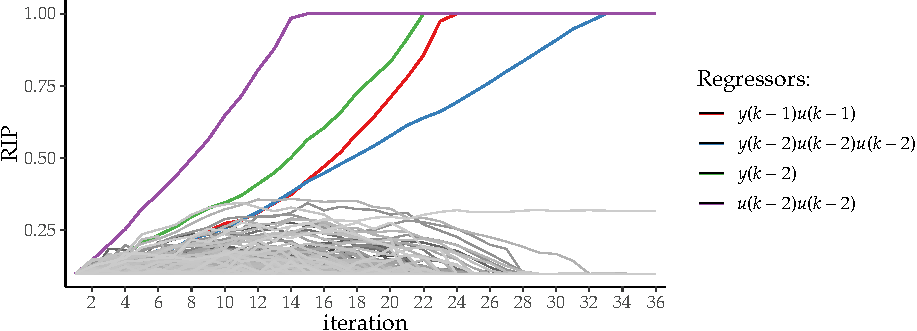
\includegraphics{./Figs/Cap3/ex31_ripsEvol.tex.pdf}
    \caption{Convergence of RIPs considering a particular realization.}
    \label{fig:ex31_rips}
  \end{figure}
  
  % Uma análise mais geral, que leva em conta o comportamento em 100 realizações é mostrado na Figura \ref{fig:ex31_density}. Neste caso observa-se que o comportamento anterior permanece na média, sendo que os regressores $y(k-1)u(k-1)$ e $y(k-2)$ são escolhidos com intervalos próximos, em média.
  A more general analysis, which takes into account the behavior in 100 realizations, is shown in Figure \ref{fig:ex31_density}. In this case it is observed that the previous behavior remains in the average.
  
  \begin{figure}[H]
    \centering
    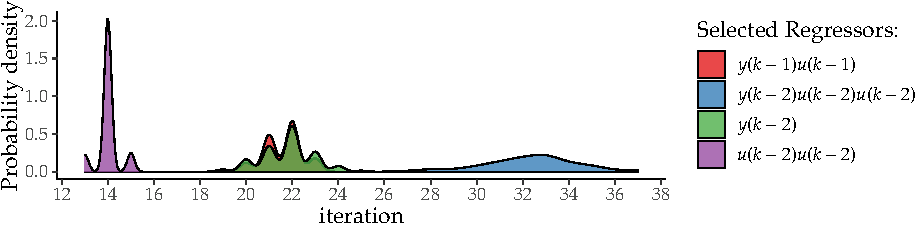
\includegraphics{./Figs/Cap3/ex31_density.tex.pdf}
    \caption{Probability density for convergence of RIPs, considering 100 realizations.}
    % COMTEMP \todo[inline]{Colocar linha de \textit{threshold} na ref{fig:RIPs1}? Mudar cores. Tentar mudar nome dos regressores (índices). Mas com certeza, mudar nomes de y para u.}
    \label{fig:ex31_density}
  \end{figure}

  % Note que os gráficos consideram somente até a 36a iteração. Isto ocorre devido ao critério de parada adotado, que interrompe o procedimento assim que as variações nos RIPs se tornam menor que um certo valor predefinido.
  Note that the graphs only consider up to the 36th iteration. This is due to the adopted stopping criteria, which interrupts the procedure as soon as the variations in the RIPs become less than a certain predefined value.
  % Ressalta-se que em todas as simulações o procedimento parou antes da 100a iteração selecionando exatamente os regressores originais, indicando que há sempre uma convergência para estes valores.
  In all simulations the procedure stopped before the 100th iteration, selecting exactly the original regressors, indicating that there is always a convergence for these values in this exemple.

% Densidade de probabilidade para convergência dos RIPs, considerando-se 100 realizações.
\end{exmp}



% \section{Control perfomance criteria}

% Como o objetivo deste trabalho é lidar com identificação e escolha de estruturas com o auxílio de estratégias VRFT, a serem aboradadas no capítulo \ref{cap:VRFT}, alguns conceitos necessários são apresentados nesta seção.
%
% Um elemento fundamental para projeto e análise de controladores na teoriade controle baseada em otimização, como é o caso do VRFT, é o conceito de \textit{desempenho de controle}. Na forma geral, este conceito pode ser expresso como a solução de um problema definido como
% \begin{equation}
%    \min_{\bm{\theta}} J(\bm{\theta}),
% \end{equation}
% onde $\vtheta \in \bm{R}$ é um vetor de $N$ parâmetros adotado como variável decisão e $J(\vtheta)$ é uma \textit{função de custo}\footnote{Outros termos também são conhecidos na literatura, como \textit{índice (ou função) de desempenho}, ou ainda, \textit{função objetivo}.}. Quanto menor o valor de $J$, melhor o desempenho segundo o critério adotado. Dependendo do objetivo de controle ou até mesmo por questões de garantias analíticas de estabilidade, diferentes funções de custo podem ser adotadas. Uma abordagem muito comum é escolher uma função de custo baseada na  norma-2 quadrática média\footnote{A norma-2 de um sinal discreto, ou vetor, $x(k)$ é definida como $||x(k)|| \triangleq \sqrt{ \sum_{k=1}^{N} [x(k)]^{2} }$. Elevando esse valor ao quadrado temos a norma-2 quadrática, que representa a energia do sinal que, dividida pelo número de amostras, como em \eqref{eq:H2}, resulta em sua energia média.}
% na forma
% \begin{equation}
%    ||x(k)||^{2} =\frac{1}{N}\sum_{k=1}^{N} \left[ x(k) \right]^{2} \triangleq \bar{\E} \left[ x(k) \right]^{2}
%    \label{eq:H2}
% \end{equation}
% em que $x(k)$ representa uma função genérica, $N$, o número de amostras e $\bar{\E}\left[ \cdot \right] $, um operador definido como
% \begin{equation}
%    \bar{\E}[x(k)] \triangleq \frac{1}{N}\sum_{k=1}^{N} [x(k)],
% \end{equation}
% que representa o cálculo da média amostral, e será usado no decorrer do texto em substituição ao somatório, por conveniência.
%
% O critério apresentado em \eqref{eq:H2} é conhecido como \textit{critério de desempenho} $H_2$ e é o que se adota neste trabalho e, para fins de objetividade, será o único abortado neste texto.
%
% O critério  $H_2$, para fins de controle, é definido de acordo com o objetivo de controle. Estes objetivos, em geral, são adotados como: (1) rastreamento de referência, (2) rejeição de ruídos e (3) economia de esforço de controle. Critérios mistos adotando mais de um destes objetivos, podem também ser definidos, como é o caso do (4) composite performance criteria. As próximas seções tratam destes critérios com um pouco mais de detalhes.

\section{Control System Setup and Notations}%
\label{sec:system_setup_}

% Nesta seção apresenta-se o sistema em malha fechada considerado, definindo as equações para seus componentes e introduzindo a notação utilizada ao longo do texto. Como pretende-se lidar com sistemas não lineares, adota-se a notação apresentada em \cite{campi2006}. Quando lidando com sistemas lineares, porém, esta notação pode parecer mais pesada que o necessário e uma notação mais usual pode ser adotada. Essas notações, são apresentadas no escopo do sistema de controle considerado e são detalhadas nas próximas subseções.
In this section, we present the closed-loop system considered, defining the equations for its components and introducing the notation used throughout the text. As it is intended to deal with non-linear systems, the notation presented in \cite{campi2006} is adopted. When dealing with linear systems, however, this notation may appear to be heavier than necessary and a more usual notation may be adopted. These notations are presented within the scope of the control system considered and are detailed in the next subsections.

\subsection{The control system}
\label{sub:o_sistema_de_controle}

% Considera-se um sistema de controle clássico do tipo SISO de um grau de liberdade, que pode ou não se encontrar sobre efeito de ruídos no sinal de saída. A Figura \ref{fig:diagrama_MF} apresenta o diagrama de blocos deste sistema, onde $C(q, \bm{\theta}, e)$ representa o Controlador, função do vetor de parâmetros $\bm{\theta}$ e $P(q,u)$, o modelo do processo, ou planta, que pode ser ou não conhecido. Os sinais $r(k)$,
It is considered a classic control system of the SISO type with a degree of freedom, which may or may not be under the effect of noise in the output signal. Figure \ref{fig:diagram_MF} shows the block diagram of this system, where $C(q, \bm{\theta}, e)$ represents the controller, a function of the vector of parameters $\bm{\theta}$ and $P(q,u)$, the process model, or plant, which may or may not be known. $r(k)$ 
\todo{Corrigir aqui. Usar somente P e C no diagrama e corrigir neste parágrafo} 
% $u(k)$, $\nu(t)$, $e(k)$, $y(k)$, e $y_\nu(k)$ são, respectivamente, os sinais de referência, controle, ruído, erro rastreamento, saída do processo e, por último, saída com ruído (ou sinal medido).
 $u(k)$, $\nu(t)$, $e(k)$, $y(k)$, and $y_\nu(k)$ are, respectively, the reference, control, noise, tracking error, process output and, finally, noise output signals.

\begin{figure}[htpb] 
   \centering
   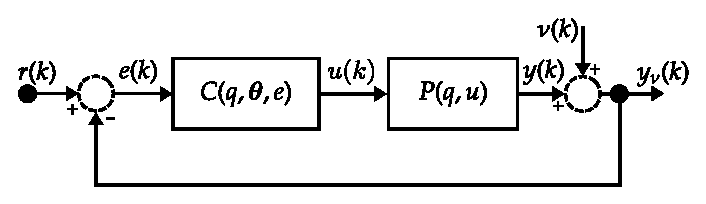
\includegraphics[width=0.8\textwidth]{Figs/diagrama_mf.eps}
   \todo[inline]{Mudar $e(k), u(k), y(k)$ e $y_{\nu}$, para $e_\theta(k), u_\theta(k), y_{\theta\nu}(k)$? Terei que mudar no texto também. Vide \ref{ass:noiseFree}.} 
   \caption{Sistema de controle.}
   \label{fig:diagrama_MF}
\end{figure}

\subsection{The process}%
\label{sec:TheProcess}

% O processo, ou planta, $P$ é um processo não-linear discreto no tempo do tipo SISO, com dinâmica não linear descrita como
The process, or plant, $P$ is a discrete non-linear time process of the SISO type, with nonlinear dynamics described as
\begin{equation}
   y(k)=p\left(y(k-1), \ldots, y(k-n_{P y}), u(k-1), \ldots, u(k-n_{P u})\right),
   \label{eq:yknl}
\end{equation}
% onde $p$ é uma função representando o processo, $n_{P y}$ é o máximo atraso na saída, $n_{P u}$ é o máximo atraso na entrada e $k$ o índice temporal.
where $p$ is a function representing the process, $n_{P y}$ is the maximum delay in the output, $n_{P u}$ is the maximum delay in the input and $k$ the temporal index.

% Por simplificação, é considerado que o atraso de tempo puro de $u$ para $y$ em $P$ é 1, mas o procedimento pode ser estendido sem problemas para atrasos maiores.
For simplicity, the pure time delay from $u$ to $y$ in $P$ is considered to be 1, but the procedure can be extended without problems for longer delays.

% Considera-se $P$ como um mapa não-linear que opera de $\mathbb{R}^{N}$ para $\mathbb{R}^{N}$. Quando sujeito às condições iniciais $i.c.= (y(0), \ldots, y(1-n_{P y}), u(-1), \ldots, u(1-n_{P u}) )$ e a um sinal de entrada no intervalo $[0, N-1]$ definido como $u(0{:}N-1) \triangleq [u(0) \cdots u(N-1)]^{T}$, $P$ gera uma saída dada por
  $P$ is considered a non-linear map that operates from $\mathbb{R}^{N}$ to $\mathbb{R}^{N}$. When subject to the initial conditions $i.c.= (y(0), \ldots, y(1-n_{P y}), u(-1), \ldots, u(1-n_{P u}) )$ and an input signal in the range $[0, N-1]$, defined as $u(0{:}N-1) \triangleq [u(0) \cdots u(N-1)]^{T}$, $P$ generates an output given by
\begin{equation}
   y(1{:}N) = P[u(0{:}N-1), \text { i.c. }].
\label{eq:Pnl}
\end{equation}

The following hypotheses are adopted:
\begin{assum}[ Process smoothness ]\label{ass:psuave}
   % A função $p$ que representa o processo é suave.
   The function $p$ that represents the process is smooth.
\end{assum}
\begin{assum}[ Uniqueness of the solution ]\label{ass:invert}
   % Para quaisquer condições iniciais dadas, se $u_{1}(0{:}N-1) \neq u_{2}(0{:} N-1)$, então $P\left[u_{1}(0{:} N-1), i . c .\right] \neq P\left[u_{2}(0{:} N-1), i . c\right]$.
   For any initial conditions given, if
   $u_{1}(0{:}N-1) \neq u_{2}(0{:} N-1)$, so $P\left[u_{1}(0{:} N-1), i . c .\right] \neq P\left[u_{2}(0{:} N-1), i . c\right]$.
\end{assum}

% A hipótese~\ref{ass:psuave} garante a invertibilidade do mapa $P$. A invertibilidade de $P$ para um sinal de entrada definido no intervalo $\left[ 0{:}N-1 \right]$
% implica na invertibilidade do mapa em um intervalo $[0{:}T]$, com $T\le N-1$ \citep{campi2004}.
The Assumption~\ref{ass:psuave} guarantees the invertibility of the $P$ map. The invertibility of $P$ for an input signal defined in the range $\left[ 0{:}N-1 \right]$
implies in the invertibility of the map in a range $[0{:}T]$, with $T\le N-1$ \citep{campi2004}.
% COMTEMP \todo{Ref.\ aqui --olhar \citep{campi2006}.} 

% COMTEMP \todo[inline]{Acabar aqui.} 

\subsection{The controller}%
\label{sub:o_controlador}

% O controlador considerado, assim como o processo, é representado por um modelo não-linear (que pode também ser linear). Para fins de identificação dos parâmetros pelo método VRFT, assunto abordado no capítulo \ref{cap:VRFT}, assume-se que uma estrutura (ou classe) é previamente escolhida. Este controlador pode ser descrito como
The controller considered, as well as the process, is represented by a non-linear model (which can also be linear). For the purpose of identifying the parameters by the VRFT method, subject addressed in the chapter \ref{cap:VRFT}, it is assumed that a structure (or class) is previously chosen. This controller can be described as
\begin{equation}
   u(k)=c\left(u(k-1), \ldots, u(k-n_{C u}), e(k), \ldots, e(k-n_{C e})\right),
\label{eq:uknl}
\end{equation}
% em que $n_{Cu}$ e $n_{Ce}$ são os máximos atrasos no sinal de controle (saída do controlador e no sinal de erro de rastreamento (entrada do controlador).
where $n_{Cu}$ and $n_{Ce}$ are the maximum delays in the control signal (controller output and tracking error signal (controller input).

% Assim como para o processo, o controlador é sujeito às condições iniciais $i.c.= u(-1), \ldots, u(-n_{C u}), e(-1), \ldots, e(-n_{C e})$
As for the process, the controller is subject to the initial conditions $$i.c.= u(-1), \ldots, u(-n_{C u}), e(-1), \ldots, e(-n_{C e})$$
% e quando alimentado com o sinal de erro $e(0{:}N-1)$, gera o sinal de controle $u(0{:}N-1)$, que é representado por
and when fed with the error signal $e(0{:}N-1)$, it generates the control signal $u(0{:}N-1)$, which is represented by
\begin{equation}
   u(0{:}N-1)=C[e(0{:}N-1), i.c.].
\label{eq:Cnl}
\end{equation}

% Neste trabalho, um dos objetivos é selecionar um controlador adequado dada uma classe fixa de controladores pelo método VRFT, conforme abordado no capítulo \ref{cap:VRFT}. Essa classe é formada por todos controladores parametrizados por
In this work, one of the objectives is to select a suitable controller given a fixed class of controllers by the VRFT method, as discussed in the chapter \ref{cap:VRFT}. This class is formed by all controllers parameterized by
\begin{equation}
   u(k)=c\left(u(k-1), \ldots, u(k-n_{C u}), e(k), \ldots, e(k-n_{C e}); \bm{\theta}\right),
\label{eq:uknl_par}
\end{equation}
% sendo $\bm{\theta} \in \mathbb{R}^{n_\theta}$ um vetor de $n_{\theta}$ parâmetros. O controlador parametrizado por $\bm{\theta}$ será aqui indicado por $C_{\theta}$, e o sinal de controle \eqref{eq:uknl} fica na forma
being $\bm{\theta} \in \mathbb{R}^{n_\theta}$ a vector of $n_{\theta}$ parameters. The controller parameterized by $\bm{\theta}$ will be indicated here by $C_{\theta}$, and the control signal \eqref{eq:uknl} is in the form
\begin{equation}
   u_{\theta}(0{:}N-1)=C_{\theta}[e(0{:}N-1), i.c.],
\label{eq:utheta}
\end{equation}
with
\begin{equation}
   e(0{:} N-1)\triangleq r(0{:} N-1)-y(0{:} N-1),
\label{eq:erro}
\end{equation}
representing the tracking error.

The following assumption is assumed for the controller:
\begin{assum}
   % O controlador $c(k)$ é uma função escalar \textit{suave} do vetor de parâmetros $\bm{\theta}$, de $u(k-1:k-n_{Cu})$  e de $e(k-0:k-n_{Ce})$, ou de forma simplificada
   % O controlador $c$ é representado por uma função escalar parametrizada como em \eqref{eq:uknl_par}, e assumido suave, ou de forma simplificada
   The $c$ controller is represented by a scalar function parameterized as in \eqref{eq:uknl_par}, and assumed to be smooth, or in a simplified way
   \begin{equation}
      c:\mathbb{R}^{n_{Cu}+n_{Ce}+1+n_{\theta}} \mapsto \mathbb{R} \text{ is smooth}.
      \label{eq:assumcon}
   \end{equation}
\end{assum}



\subsection{The feedback system}%
\label{sub:o_sistema_realimentado}

% As interconexões do sistema em malha fechada apresentado na Figura \ref{fig:diagrama_MF}, juntamente com as equações do processo \eqref{eq:Pnl} e do controlador \eqref{eq:Cnl} resultam na relação
The interconnections of the closed-loop system shown in Figure \ref{fig:diagrama_MF}, together with the equations of the process \eqref{eq:Pnl} and the controller \eqref{eq:Cnl} result in the relationship
\begin{align}
   y(1: N) &=P[u(0{:} N-1), i . c .] \nonumber \\
   &=P[C[e(0{:} N-1), i . c .], i . c .]
   \label{eq:CLSnl}
\end{align}

\subsection{Notation simplification}%
\label{sub:simplificações_nas_notações}

% Por simplificações nas notações, considera-se as condições iniciais da planta e do controlador nulas. Tal requerimento não é necessário, porém só leva  a complicações desnecessárias, principalmente na notação. Além do mais, se as N é grande o suficiente, as condições iniciais influenciam pouco para casos estáveis.
For simplifications in the notations, the initial conditions of the plant and the controller are considered null. Such a requirement is not necessary, but it only leads to unnecessary complications, especially in the notation. Furthermore, if the N is large enough, the initial conditions have little influence on stable cases.
% Além disso, os argumentos temporais são omitidos, resultando no uso dos símbolos: $u$ para representar $u(0{:}N-1)$, $r$ para $r(0{:}N-1)$, $e$ para $e(0{:}N-1)$ e  $y$ para $r(1{:}N)$. Note o avanço temporal de $y$ em relação às outras variáveis. Desta forma, representa-se  $y(0{:}N)$ é representado por $Dy$, sendo $D$ uma matriz nilpotente de deslocamento em atraso definida como
In addition, time arguments are omitted, resulting in the use of the symbols: $u$ to represent $u(0{:}N-1)$, $r$ for $r(0{:}N-1)$, $e$ for $e(0{:}N-1)$ and $y$ for $r(1{:}N)$. Note the time advance of $y$ in relation to the other variables. In this way, $y(0{:}N)$ is represented by $Dy$, with $D$ being a nilpotent delay displacement matrix defined as
\begin{equation}
   D \triangleq \begin{bmatrix} 
      0 & 0 & \dots & 0 & 0 \\
      1 & 0 & \dots & 0 & 0 \\
      0 & 1 & \dots & 0 & 0 \\
      \vdots & \vdots & \ddots & \vdots & \vdots \\
      0 & 0 & \dots & 1 & 0 \\
   \end{bmatrix} 
\label{eq:}
\end{equation}

% Com isso, \eqref{eq:CLSnl} pode ser rescrita como
With that, \eqref{eq:CLSnl} can be written as
\begin{equation}
   y = P[C[r-Dy]]
   \label{eq:ymf}
\end{equation}
% Ou, utilizando o controlador parametrizado de \eqref{eq:utheta},
Or, using the  parametrized controller \eqref{eq:utheta},
\begin{equation}
   y_{\theta} = P[C_{\theta}[r-Dy_{\theta}]]
   \label{eq:ytheta}
\end{equation}


\subsection{The control objective}%
\label{sub:the_reference_model}

% Um elemento fundamental para projeto e análise de controladores na teoriade controle baseada em otimização, como é o caso do VRFT, é o conceito de \textit{desempenho de controle}. Na forma geral, este conceito pode ser expresso como a solução de um problema definido como
A fundamental element for controller design and analysis in optimization-based control theory, as is the case with VRFT, is the concept of \textit{control performance}. In general, this concept can be expressed as the solution to a problem defined as
\begin{equation}
   \min_{\bm{\theta}} J(\bm{\theta}),
\end{equation}
% onde $\vtheta \in \mathbb{R}$ é um vetor de $n_{\theta}$ parâmetros adotado como variável decisão e $J(\bm{\theta})$ é uma \textit{função de custo}\footnote{Outros termos também são conhecidos na literatura, como \textit{índice (ou função) de desempenho}, ou ainda, \textit{função objetivo}.}. Quanto menor o valor de $J(\bm{\theta})$, melhor o desempenho segundo algum critério adotado. Dependendo do objetivo de controle, ou até mesmo por questões de garantias analíticas de estabilidade, diferentes funções de custo podem ser adotadas. Uma abordagem muito comum é escolher uma função de custo baseada na  norma-2 quadrática média\footnote{A norma-2 de um sinal discreto, ou vetor, $x(t)$ é definida como $||x(t)|| \triangleq \sqrt{ \sum_{t=1}^{N} [x(t)]^{2} }$. Elevando esse valor ao quadrado temos a norma-2 quadrática, que representa a energia do sinal que, dividida pelo número de amostras, como em \eqref{eq:H2}, resulta em sua energia média.}
onde $\vtheta \in \mathbb{R}$ é um vetor de $n_{\theta}$ parâmetros adotado como variável decisão e $J(\bm{\theta})$ é uma \textit{função de custo}\footnote{Outros termos também são conhecidos na literatura, como \textit{índice (ou função) de desempenho}, ou ainda, \textit{função objetivo}.}. Quanto menor o valor de $J(\bm{\theta})$, melhor o desempenho segundo algum critério adotado. Dependendo do objetivo de controle, ou até mesmo por questões de garantias analíticas de estabilidade, diferentes funções de custo podem ser adotadas. Uma abordagem muito comum é escolher uma função de custo baseada na  norma-2 quadrática média\footnote{A norma-2 de um sinal discreto, ou vetor, $x(t)$ é definida como $||x(t)|| \triangleq \sqrt{ \sum_{t=1}^{N} [x(t)]^{2} }$. Elevando esse valor ao quadrado temos a norma-2 quadrática, que representa a energia do sinal que, dividida pelo número de amostras, como em \eqref{eq:H2}, resulta em sua energia média.}
na forma
\begin{equation}
   ||x(k)||^{2} =\frac{1}{N}\sum_{k=1}^{N} \left[ x(k) \right]^{2} \triangleq \bar{\E} \left[ x(k) \right]^{2}
   \label{eq:H2}
\end{equation}
em que $x(k)$ representa uma função genérica, $N$, o número de amostras e $\bar{\E}\left[ \cdot \right] $, um operador definido como
\begin{equation}
   \bar{\E}[x(k)] \triangleq \frac{1}{N}\sum_{k=1}^{N} [x(k)],
\end{equation}
que representa o cálculo da média amostral, e será usado no decorrer do texto em substituição ao somatório, por conveniência.

O critério apresentado em \eqref{eq:H2} é conhecido como \textit{critério de desempenho} $H_2$ e é o que se adota neste trabalho e, para fins de objetividade, será o único abortado neste texto.

O critério  $H_2$, para fins de controle, é definido de acordo com o objetivo de controle. Estes objetivos, em geral, são adotados como: (1) rastreamento de referência, (2) rejeição de ruídos e (3) economia de esforço de controle. Critérios mistos adotando mais de um destes objetivos, podem também ser definidos, como é o caso do (4) composite performance criteria. As próximas seções tratam destes critérios com um pouco mais de detalhes.


\subsubsection{The Reference Tracking Objective}%
\label{sub:the_reference_tracking_objective}
Um dos principais objetivos do controle em malha fechada é fazer com que o sinal controlado siga um sinal de referência desejado, de modo que sejam o mais próximo possível. Desprezando-se o efeito do ruído na saída, e considerando um controlador parametrizado, a resposta do sistema em malha fechada é dada por \eqref{eq:ytheta}.

Esse objetivo pode ser traduzido como a minimização de uma função custo dada pela norma-2 do erro de rastreamento, na forma
\begin{equation}
   % J(\bm{\theta}) = \bar{\E}\left[ r(t) - y_r(t,\bm{\theta}) \right].
   J_r^N(\bm{\theta}) \triangleq || r - y_\theta ||^2 .
   \label{eq:Jr}
\end{equation}
% onde o operador $\bar{\E}\left[ \cdot \right] $ (operador de média amostral), é definido como
% \begin{equation}
% \bar{\E}[\cdot] \triangleq \frac{1}{N}\sum_{k=1}^{N} [\cdot]^{2},
% \end{equation}
% e será usado no decorrer do texto em substituição ao somatório por conveniência.

\subsubsection{The Reference Model Objective}%
\label{sub:The Reference Model Objective}

Um fato bem conhecido na comunidade de controle é que na prática é impossível fazer com que a saída siga perfeitamente o sinal de referência durante todo o tempo, ou seja \eqref{eq:Jr} nunca será zero.
Para contornar esse fato uma saída é relaxar o objetivo de rastreamento por outro que satisfaça pré-requisitos desejados (como tempo de acomodação, instante de pico, sobressalto máximo, dentre outros), mas que seja menos exigente que a referência original.

Esse novo objetivo é traduzido para um modelo conhecido como \textit{modelo de referência} representado aqui por um mapa de $\mathbb{R}^{N}$ para $\mathbb{R}^{N}$, que mapeia um sinal de referência, digamos, $\tilde{r}$ para um sinal de saída $\tilde{y}$ com um comportamento desejado\footnote{o símbolo \ $\tilde{}$ \ enfatiza que estes sinais são para o modelo de referência.}.
\begin{equation}
   M:\tilde{r} \in \mathbb{R}^N \mapsto \tilde{y} \in \mathbb{R}^N
\label{eq:Mmap}
\end{equation}
Este mapa, a princípio pode ser um modelo não linear, desde que seja suave e invertível. Porém, em geral, por conveniência, é escolhido como um modelo linear, mas ainda sim deve ser invertível. Defini-se a seguinte hipótese:
\begin{assum}[Invertibilidade do modelo de referência]
   $M$ é triangular inferior e invertível.
\end{assum}
O fato de $M$ ser adotado como triangular inferior garante que será causal, com atraso puro maior ou igual a 1.
Um exemplo de escolha típica para $M$, para o caso linear, é o filtro
\begin{equation}
   M(q)=\frac{b_{1} q^{-1}+\cdots+b_{n_{M r}} q^{-n_{M r}}}{1+a_{1} q^{-1}+\cdots+a_{n_{M y}} q^{-n_{M y}}}
\label{eq:Mq}
\end{equation}
sendo $n_{Mr}$ e $n_{My}$ os máximos atrasos pra a referência e para a saída, respectivamente, e $q$ um operador de atraso. No domínio do tempo, \eqref{eq:Mq} corresponde a 
\begin{align}
   \label{eq:ytMr}
   \tilde{y}(k)=-a_{1} \tilde{y}(k-1)-\cdots &-a_{n_{M y}} \tilde{y}\left(k-n_{M y}\right) +b_{1} \tilde{r}(k-1)+\cdots+b_{n_{M r}} \tilde{r}\left(k-n_{M r}\right)
\end{align}

Uma vez definido o modelo de referência que traduz o comportamento desejado em malha fechada, o novo objetivo de controle é traduzido como

   % e será, neste texto, referido como $M(z)$, quando na forma de função de transferência (linear) ou $M(q)$ quando na forma de modelos temporais (linear ou não linear), ou simplesmente $M$ quando na forma apresentada na section \ref{sec:}. Neste sentido, uma nova função de custo é definida como
\begin{equation}
   J_{RM}^N(\bm{\theta}) \triangleq \left\lVert y_\theta - \tilde{y} \right\lVert^{2} = \left\lVert P[C_\theta[\tilde{r}-Dy_\theta]] - M[\tilde{r}] \right\lVert^{2}
   % J_{RM}^N(\bm{\theta}) \triangleq \bar{\E}\left[ y_r(k,\bm{\theta}) - y_{RM}(k) \right]^{2} = \bar{\E}\left[ T(q,\bm{\theta},r(k)) - M(q,r(k)) \right]^{2}
   \label{eq:Jy}
\end{equation}
sendo $\tilde{y} = M[\tilde{r}]$ o sinal de saída do modelo de referência desejado, quando sobre efeito de um sinal de referência $r$. Tal critério é conhecido como \textit{critério do modelo de referência}.


\subsubsection{The Noise Rejection Objective}%
\label{sub:the_noise_rejection_objective}

Outro objetivo comum em sistemas de controle é minimizar o efeito do ruído no sinal de saída. O sinal de saída devido somente a atuação do sinal de ruído no processo pode ser escrito como
\begin{equation}
   y_{\theta\nu}(\bm{\theta}) \triangleq S_\theta[\nu] = \nu-P[C_\theta[Dy_{\theta\nu}],
\end{equation}
em que $\nu \triangleq \nu(0{:}N)$ representa o sinal de ruído e $S_{\theta}$ um mapa de ruído para a saída do processo, ou seja $M:\nu \mapsto y_{\theta\nu}$, que, para o caso linear, é também conhecido como função sensibilidade. Quando analisada a magnitude deste sinal em função de alguma norma, tem-se o critério de desempenho de rejeição de ruído $J_\nu^N(\bm{\theta})$ que, utilizando a norma-2, é dado por
\begin{equation}
   J_\nu^N(\bm{\theta}) \triangleq \norm{ y_{\theta\nu} }^2 = \norm{ S_\theta[\nu] }^2.
   \label{eq:Jnoise}
\end{equation}

Assim como no caso do rastreamento, não é possível a eliminação completa do efeito do ruído e um relaxamento neste critério é desejável, pelos mesmos motivos. Neste caso é definida uma função sensibilidade desejada $S_{M}$\footnote{O índice $M$ é utilizado para manter a analogia com o índice utilizado pelo modelo de referência para o caso de rastreamento.} e adota-se o critério
\begin{equation}
   J_{RM\nu}^N(\bm{\theta}) \triangleq  \norm{S_\theta[\nu] - S_M[\nu]}^{2}.
   \label{eq:JeRM}
\end{equation}





\subsubsection{The Economy of Control Effort Objective}%
\label{sub:the_economy_of_control_effot_objective}

Um objetivo comum no projeto de controladores, principalmente na área de controle ótimo, é a minimização do esforço de controle. Para minimizar o sinal de controle o seguinte índice pode ser definido:
\begin{equation}
   J_u^N(\bm{\theta}) \triangleq \norm{ u(k) }^{2},
   \label{eq:Ju}
\end{equation}
sendo $u(k)$ o sinal de controle. Porém este índice não deve ser usado sozinho, uma vez que $J_u^N(\bm{\theta}) = 0$ implicaria em $u \equiv 0$. Portanto o que se faz é utilizar-se de uma combinação deste índice, com outros, por exemplo, com o objetivo de rastreamento de referência, resultando em 
\begin{equation}
   J_\lambda^N = J_{RM}^N(\bm{\theta}) + \lambda J_u^N(\bm{\theta})
   \label{eq:Jl}
\end{equation}
em que $\lambda \in \mathbb{R}$ representa um parâmetro de ajuste.
Ao se utilizar de controladores baseados em modelo de referência, como o caso do VRFT a ser visto no \ref{cap:VRFT}, um efeito de economia de esforço de controle pode ser obtido ao se escolher um modelo de referência adequado. Portanto, neste trabalho a inclusão do índice \eqref{eq:Ju} na função de custo é desconsiderado.



\subsubsection{The Composite Performance Objective}%
\label{sub:the_composite_performance_objective}

Outro objetivo, mais realista que o de rastreamento de referência, é o \textit{composite performance}, que objetiva tanto reduzir o erro de rastreamento quanto rejeitar efeitos do ruído na saída. Este critério é dado por
\begin{equation}
   J_T^N(\bm{\theta}) \triangleq \norm{ y_{\theta\nu} - \tilde{y} }^2,
   \label{eq:JT}
\end{equation}
em que, diferentemente de $\tilde{y}$ em \eqref{eq:Jy}, o sinal $y_{\theta\nu}= P[C_\theta[r-y_\theta]] + S[\nu]$ depende do ruído. O critério final será a soma dos dois critérios anteriores, uma vez que a referência e o ruído são sinais independentes estatisticamente e pode ser escrito como

\begin{equation}
   J_T^N(\bm{\theta}) = \norm{ P[C_\theta[r-Dy_\theta]] - M[r] }^{2} + \norm{ S[\nu] }^2.
   \label{eq:}
\end{equation}






\section{The Ideal Controller}%
\label{sec:ideal_controller}
% COMTEMP \todo{Tirar o ``Matched Control??''.}

Considerando o sistema realimentado apresentado em \eqref{eq:ymf}, e assumindo a invertibilidade de $P$ e que $M$ é triangular inferior, resolvendo \eqref{eq:ymf} para $C$, é possível calcular o controlador ideal, que resulta nos parâmetros ótimos para $C_\theta$, desde que $C_\theta$ tenha mesma estrutura (ou pertença à mesma classe) do controlador ideal. Este controlador ideal é definido como:
\begin{equation}
   C_0 \triangleq P^{-1}(I-MD)^{-1}M,
\label{eq:}
\end{equation}
onde $I$ é a matriz identidade e $C^{i}$ é o controlador ideal.

Quando o $C_0$ é usado na malha fechada, o mapa de $r$ para $y$ é dado por $M$, ou seja, $y=M[r]$

Para o caso linear SISO (Single Input Single Output), se o modelo do processo é conhecido e considerando que este é de 
% \todo{[DONE] Falar aqui (citar) do trabalho da Lucíola no sentido de lidar com fase não mínima. Talvez citar Stogestad também.}
fase mínima, o controlador ideal $C_0$ pode ser escrito na forma de função de transferência como
\begin{equation}
   C_0(z) = \frac{M(z)}{P(z)\left(1-M(z)\right)},
   \label{eq:Cdz}
\end{equation}
em que $P(z)$ e $M(z)$ representam respectivamente as funções de transferência do processo e do modelo de referência.

Note que, se o processo é de fase não mínima, devido a zeros fora do círculo unitário no plano-$z$, a inversa de $P(z)$ em \eqref{eq:Cdz} resulta em instabilidade do sistema. Soluções para este problema têm sido apresentadas há décadas para projetos MBC, como por exemplo regras para sintonia de PID, como a desenvolvida por \cite{skogestad2003}.
Uma abordagem no mais recente, no âmbito do DDC, é apresentada por \cite{campestrini2011}.
% COMTEMP \todo{Colocar um pouco mais sobre esteartigo aqui.} 


% COMTEMP \todo[inline]{Colocar aqui a respeito do caso não linear, como em \cite[p. 19]{campi2006}, mas antes introduzir notação.}





